\documentclass[10pt, notes]{beamer}

\usepackage[utf8x]{inputenc}
\usepackage[T1]{fontenc}
\usepackage{lmodern}
\usepackage{microtype}
\usepackage{xspace}
%\usepackage[binary-units=true]{siunitx}
\usepackage{graphicx}
\usepackage{hyperref}
\usepackage{todonotes}
\usepackage{epstopdf}
\usepackage{array}
\usepackage{multicol}
\usepackage{multirow}
\usepackage{tabularx} 	% tabular with automatic line-break
\newcolumntype{Y}{>{\centering\arraybackslash}X} % centered column
\usepackage{amsmath}
\usepackage{grffile} 	% better name handling with graphicx
\usepackage{currfile} 	% provides relative file inclusion for tikzscale

\usepackage[]{algorithm2e}

\usepackage{tikz}
\usepackage{pgfplots}
\usepackage{tikzscale}
\pgfplotsset{compat=newest}
\usetikzlibrary{plotmarks}
\usepackage[absolute,overlay]{textpos}

% Math symbols
\usepackage{amsmath}
\usepackage{amssymb}
\usepackage{amsthm}
\DeclareMathOperator*{\argmin}{arg\,min}
\DeclareMathOperator*{\argmax}{arg\,max}
\newcommand\norm[1]{\left\lVert#1\right\rVert}

% Sets
\newcommand{\Z}{\mathbb{Z}}
\newcommand{\R}{\mathbb{R}}
\newcommand{\Rn}{\R^n}
\newcommand{\Rnn}{\R^{n \times n}}
\newcommand{\C}{\mathbb{C}}
\newcommand{\K}{\mathbb{K}}
\newcommand{\Kn}{\K^n}
\newcommand{\Knn}{\K^{n \times n}}

\newcommand\eqdef{\triangleq}

% Vectors
\newcommand{\vct}[1]{\boldsymbol{#1}}
\newcommand{\va}{\vct{a}}
\newcommand{\vb}{\vct{b}}
\newcommand{\vc}{\vct{c}}
\newcommand{\vd}{\vct{d}}
\newcommand{\ve}{\vct{e}}
\newcommand{\vf}{\vct{f}}
\newcommand{\vg}{\vct{g}}
\newcommand{\vh}{\vct{h}}
\newcommand{\vi}{\vct{i}}
\newcommand{\vj}{\vct{j}}
\newcommand{\vk}{\vct{k}}
\newcommand{\vl}{\vct{l}}
\newcommand{\vm}{\vct{m}}
\newcommand{\vn}{\vct{n}}
\newcommand{\vo}{\vct{o}}
\newcommand{\vp}{\vct{p}}
\newcommand{\vq}{\vct{q}}
\newcommand{\vr}{\vct{r}}
\newcommand{\vs}{\vct{s}}
\newcommand{\vt}{\vct{t}}
\newcommand{\vu}{\vct{u}}
\newcommand{\vv}{\vct{v}}
\newcommand{\vw}{\vct{w}}
\newcommand{\vx}{\vct{x}}
\newcommand{\vy}{\vct{y}}
\newcommand{\vz}{\vct{z}}
% Greek letter vectors
\newcommand{\valpha}{\vct{\alpha}}
\newcommand{\vbeta}{\vct{\beta}}
\newcommand{\vepsilon}{\vct{\epsilon}}
\newcommand{\vgamma}{\vct{\gamma}}
\newcommand{\vlambda}{\vct{\lambda}}
\newcommand{\vnu}{\vct{\nu}}
\newcommand{\vphi}{\vct{\phi}}
\newcommand{\vpsi}{\vct{\psi}}
\newcommand{\vtheta}{\vct{\theta}}
\newcommand{\vxi}{\vct{\xi}}
\newcommand{\vzero}{\vct{0}}
\newcommand{\vone}{\vct{1}}
% Matrices
\newcommand{\mtx}[1]{\boldsymbol{#1}}
\newcommand{\mzero}{\mtx{0}}
\newcommand{\mA}{\mtx{A}}
\newcommand{\mB}{\mtx{B}}
\newcommand{\mC}{\mtx{C}}
\newcommand{\mD}{\mtx{D}}
\newcommand{\mE}{\mtx{E}}
\newcommand{\mF}{\mtx{F}}
\newcommand{\mG}{\mtx{G}}
\newcommand{\mH}{\mtx{H}}
\newcommand{\mI}{\mtx{I}}
\newcommand{\mJ}{\mtx{J}}
\newcommand{\mK}{\mtx{K}}
\newcommand{\mL}{\mtx{L}}
\newcommand{\mM}{\mtx{M}}
\newcommand{\mN}{\mtx{N}}
\newcommand{\mO}{\mtx{O}}
\newcommand{\mP}{\mtx{P}}
\newcommand{\mQ}{\mtx{Q}}
\newcommand{\mR}{\mtx{R}}
\newcommand{\mS}{\mtx{S}}
\newcommand{\mT}{\mtx{T}}
\newcommand{\mU}{\mtx{U}}
\newcommand{\mV}{\mtx{V}}
\newcommand{\mW}{\mtx{W}}
\newcommand{\mX}{\mtx{X}}
\newcommand{\mY}{\mtx{Y}}
\newcommand{\mZ}{\mtx{Z}}

\usepackage{comment}
\usepackage{pgfpages}
\usepackage{bm}

\usetheme[progressbar=frametitle]{metropolis}
\tikzset{font={\fontsize{10pt}{12}\selectfont}}
\usepackage{hf-tikz}
\usetikzlibrary{ 
	calc,
	arrows,
	arrows.meta,
	automata, 
	shapes, 
	snakes, 
	positioning, 
	decorations,
	decorations.text,
	fit,
	matrix,
	mindmap
	}
\tikzstyle{noeud-std}=[draw,fill=black,circle,inner sep=0pt,minimum size=7pt]
\usepackage{tkz-graph}
\usepackage{xspace}
\usepackage{amsmath}
\usepackage{mathtools}

\definecolor{green}{HTML}{14B03D}
\newcommand{\payoff}[2]{{\color{green}#1}, {\color{red}#2}}


\title{LINMA2345 - Game theory}
\subtitle{Repeated games}
\date{\today}
\author{Antoine Gennart\and Jonathan Sarteel\and Antoine Paris}
\institute{Ecole polytechnique de Louvain}
\titlegraphic{\hfill
\includegraphics[height=1cm]{logo}}

\begin{document}
\maketitle

\begin{frame}{Outline}
    \setbeamertemplate{sections in toc}[sections numbered]
    \tableofcontents[hideallsubsections]
\end{frame}

\section{Finitely Repeated Games}
\begin{frame}{Outline}
    \tableofcontents[currentsection]
\end{frame}

\begin{frame}{What is a finitely repeated games?}
    In a \textit{finitely repeated game}, players
    \begin{itemize}
        \item play the same game for a finite number of times $K$,
        \textbf{known by the players before the game starts}, and
        \item collect their payoffs after each round (and thus observe what
        the others played).
    \end{itemize}

    \begin{figure}[!ht]
        \centering
        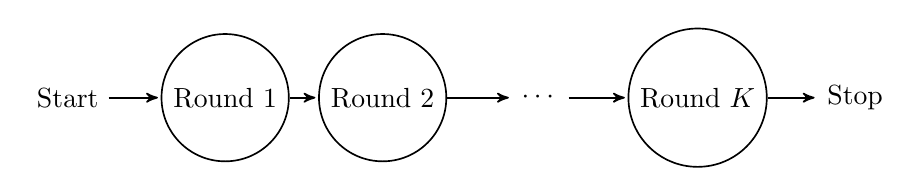
\begin{tikzpicture}[->,>=stealth',shorten >=1pt,auto,node distance=2cm, semithick, scale = 1,
            transform shape ]
            \node	        (start)								{Start};
            \node[state] 	(n1)    	[right of = start]		{Round 1};
            \node[state] 	(n2)		[right of = n1]			{Round 2};
            \node	        (dots)		[right of = n2]			{$\cdots$};
            \node[state] 	(nk)		[right of = dots]		{Round $K$};
            \node	        (stop)		[right of = nk]			{Stop};
            \path 	(start) edge node {}	(n1)
                    (n1)	edge node {}	(n2)
                    (n2)	edge node {}	(dots)
                    (dots)	edge node {}	(nk)
                    (nk) 	edge node {}	(stop);
        \end{tikzpicture}
        \caption{Finitely Repeated Games.}
    \end{figure}
\end{frame}

\begin{frame}{Let's play the Prisoner's Dilemma 2 times}
    \begin{exampleblock}{Example}
        Consider the Prisoner's Dilemma in normal form.
        \begin{table}
            \begin{tabular}{c|cc}
                & {\color{red}c}    & {\color{red}d} \\
                \hline
                {\color{green}C}    & \payoff{-1}{-1}   & \payoff{-4}{~0} \\
                {\color{green}D}    & \payoff{~0}{-4}    & \payoff{-3}{-3} 
            \end{tabular}
            \caption{Prisoner's Dilemma in normal form.}
        \end{table}
    
        \begin{itemize}
            \item The only Nash Equilibrium of this game is for both
            players to defect.
            \item Let's play this game 2 times in a row and see what happens.
        \end{itemize}
        
        \vspace{0.5cm}
        \hfill \textit{Hint}: \reflectbox{think backward}.

    \end{exampleblock}
\end{frame}

\note{
    Write the game in normal form on the blackboard as it will be used during the whole
    presentation.

    Draw a table on the blackboard and collect the actions/outcomes of each pair
    of students after each round.

    At the end, quickly compare the result. Ask students to motivate their strategy
    choice (especially if it differs from what a rational player would do).

    Probably the audience will cooperate more than expected.
}

\begin{frame}{The twice repeated Prisoner's Dilemma: Nash Equilibrium}
We proceed by \textit{backward induction} to find the Nash Equilibrium.
\begin{figure}[!ht]
    \centering
    \scalebox{0.65}{
    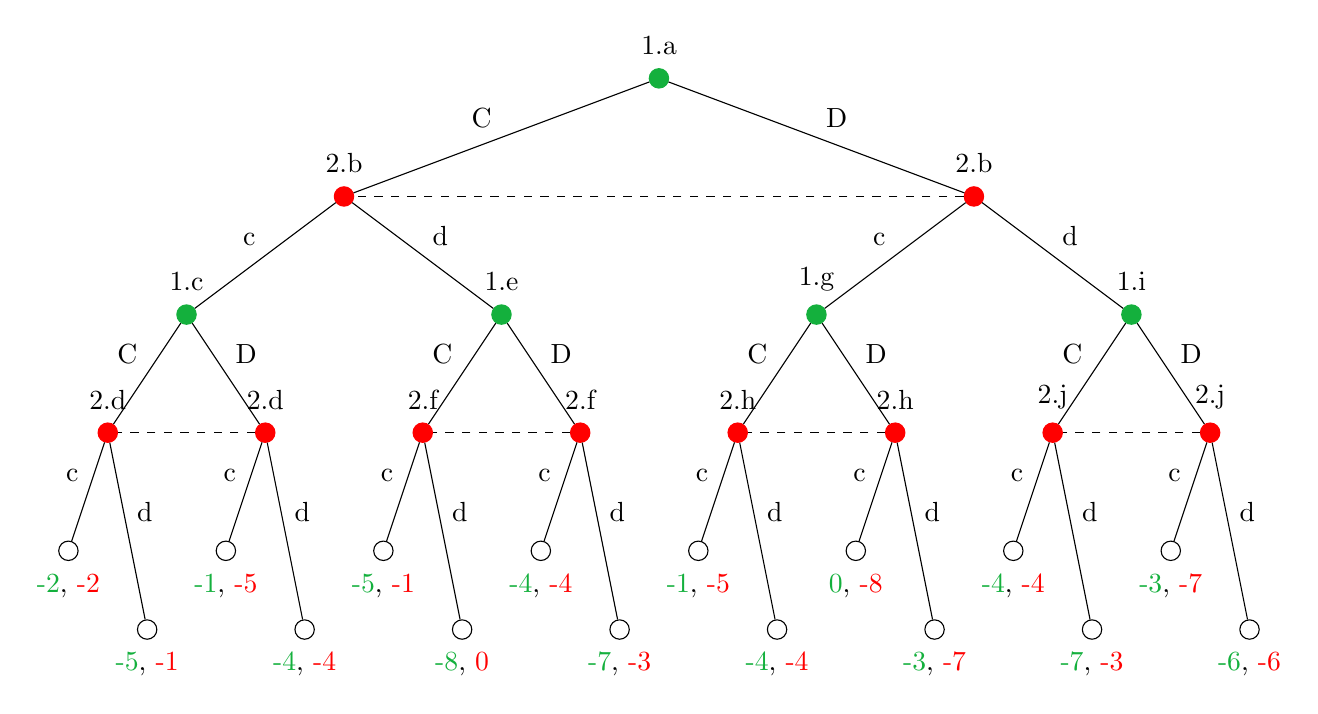
\begin{tikzpicture}
    \node[noeud-std, color=green] (n1) {}
       [sibling distance=8cm]
          child {node[noeud-std, color=red] (n2-1c) {} % 1
          [sibling distance=4cm]
                 child{node[noeud-std, color=green] (n1-1c2c){} % 2
                    [sibling distance=2cm]
                    child{node[noeud-std, color=red] (n2-1c2c1c){}  % 1
                        [sibling distance = 1cm]
                             child[level distance=1.5cm]{node[noeud-std,fill=white] (p-1c2c1c2c){} } % 1
                             child[level distance=2.5cm]{node[noeud-std,fill=white] (p-1c2c1c2d){} } % 1
                         }
                    child{node[noeud-std, color=red] (n2-1c2c1d){}  % 1
                        [sibling distance = 1cm]
                            child[level distance=1.5cm]{node[noeud-std,fill=white] (p-1c2c1d2c){} } % 1
                            child[level distance=2.5cm]{node[noeud-std,fill=white] (p-1c2c1d2d){} } % 1
                        }
                }
                child{node[noeud-std, color=green] (n1-1c2d){} % 2
                    [sibling distance=2cm]
                    child{node[noeud-std, color=red] (n2-1c2d1c){}  % 1
                        [sibling distance = 1cm]
                             child[level distance=1.5cm]{node[noeud-std,fill=white] (p-1c2d1c2c){} } % 1
                             child[level distance=2.5cm]{node[noeud-std,fill=white] (p-1c2d1c2d){} } % 1
                         }
                    child{node[noeud-std, color=red] (n2-1c2d1d){}  % 1
                        [sibling distance = 1cm]
                            child[level distance=1.5cm]{node[noeud-std,fill=white] (p-1c2d1d2c){} } % 1
                            child[level distance=2.5cm]{node[noeud-std,fill=white] (p-1c2d1d2d){} } % 1
                        }
                }
       }
       child {node[noeud-std, color=red] (n2-1d) {} % 1
          [sibling distance=4cm]
                 child{node[noeud-std, color=green] (n1-1d2c){} % 2
                    [sibling distance=2cm]
                    child{node[noeud-std, color=red] (n2-1d2c1c){}  % 1
                        [sibling distance = 1cm]
                             child[level distance=1.5cm]{node[noeud-std,fill=white] (p-1d2c1c2c){} } % 1
                             child[level distance=2.5cm]{node[noeud-std,fill=white] (p-1d2c1c2d){} } % 1
                         }
                    child{node[noeud-std, color=red] (n2-1d2c1d){}  % 1
                        [sibling distance = 1cm]
                            child[level distance=1.5cm]{node[noeud-std,fill=white] (p-1d2c1d2c){} } % 1
                            child[level distance=2.5cm]{node[noeud-std,fill=white] (p-1d2c1d2d){} } % 1
                        }
                }
                child{node[noeud-std, color=green] (n1-1d2d){} % 2
                    [sibling distance=2cm]
                    child{node[noeud-std, color=red] (n2-1d2d1c){}  % 1
                        [sibling distance = 1cm]
                             child[level distance=1.5cm]{node[noeud-std,fill=white] (p-1d2d1c2c){} } % 1
                             child[level distance=2.5cm]{node[noeud-std,fill=white] (p-1d2d1c2d){} } % 1
                         }
                    child{node[noeud-std, color=red] (n2-1d2d1d){}  % 1
                        [sibling distance = 1cm]
                            child[level distance=1.5cm]{node[noeud-std,fill=white] (p-1d2d1d2c){} } % 1
                            child[level distance=2.5cm]{node[noeud-std,fill=white] (p-1d2d1d2d){} } % 1
                        }
                }
       }

    ;
    %
    \node[above=5pt] at (n1) {1.a};
    \node[above left] at ($(n1)!{0.5}!(n2-1c)$) {C};
    \node[above right] at ($(n1)!{0.5}!(n2-1d)$) {D};

    \node[above=5pt] at (n2-1c) {2.b};
    \node[above left] at ($(n2-1c)!{0.5}!(n1-1c2c)$) {c};
    \node[above right] at ($(n2-1c)!{0.5}!(n1-1c2d)$) {d};
    \node[above=5pt] at (n1-1c2c) {1.c};
    \node[above left] at ($(n1-1c2c)!{0.5}!(n2-1c2c1c)$) {C};
    \node[above right] at ($(n1-1c2c)!{0.5}!(n2-1c2c1d)$) {D};
    \node[above=5pt] at (n2-1c2c1d) {2.d};
    \node[above left] at ($(n2-1c2c1d)!{0.5}!(p-1c2c1d2c)$) {c};
    \node[above right] at ($(n2-1c2c1d)!{0.5}!(p-1c2c1d2d)$) {d};
    \node[above=5pt] at (n2-1c2c1c) {2.d};
    \node[above left] at ($(n2-1c2c1c)!{0.5}!(p-1c2c1c2c)$) {c};
    \node[above right] at ($(n2-1c2c1c)!{0.5}!(p-1c2c1c2d)$) {d};
    \node[above=5pt] at (n1-1c2d) {1.e};
    \node[above left] at ($(n1-1c2d)!{0.5}!(n2-1c2d1c)$) {C};
    \node[above right] at ($(n1-1c2d)!{0.5}!(n2-1c2d1d)$) {D};
    \node[above=5pt] at (n2-1c2d1d) {2.f};
    \node[above left] at ($(n2-1c2d1d)!{0.5}!(p-1c2d1d2c)$) {c};
    \node[above right] at ($(n2-1c2d1d)!{0.5}!(p-1c2d1d2d)$) {d};
    \node[above=5pt] at (n2-1c2d1c) {2.f};
    \node[above left] at ($(n2-1c2d1c)!{0.5}!(p-1c2d1c2c)$) {c};
    \node[above right] at ($(n2-1c2d1c)!{0.5}!(p-1c2d1c2d)$) {d};

    \node[above=5pt] at (n2-1d) {2.b};
    \node[above left] at ($(n2-1d)!{0.5}!(n1-1d2c)$) {c};
    \node[above right] at ($(n2-1d)!{0.5}!(n1-1d2d)$) {d};
    \node[above=5pt] at (n1-1d2c) {1.g};
    \node[above left] at ($(n1-1d2c)!{0.5}!(n2-1d2c1c)$) {C};
    \node[above right] at ($(n1-1d2c)!{0.5}!(n2-1d2c1d)$) {D};
    \node[above=5pt] at (n2-1d2c1d) {2.h};
    \node[above left] at ($(n2-1d2c1d)!{0.5}!(p-1d2c1d2c)$) {c};
    \node[above right] at ($(n2-1d2c1d)!{0.5}!(p-1d2c1d2d)$) {d};
    \node[above=5pt] at (n2-1d2c1c) {2.h};
    \node[above left] at ($(n2-1d2c1c)!{0.5}!(p-1d2c1c2c)$) {c};
    \node[above right] at ($(n2-1d2c1c)!{0.5}!(p-1d2c1c2d)$) {d};
    \node[above=5pt] at (n1-1d2d) {1.i};
    \node[above left] at ($(n1-1d2d)!{0.5}!(n2-1d2d1c)$) {C};
    \node[above right] at ($(n1-1d2d)!{0.5}!(n2-1d2d1d)$) {D};
    \node[above=5pt] at (n2-1d2d1d) {2.j};
    \node[above left] at ($(n2-1d2d1d)!{0.5}!(p-1d2d1d2c)$) {c};
    \node[above right] at ($(n2-1d2d1d)!{0.5}!(p-1d2d1d2d)$) {d};
    \node[above=5pt] at (n2-1d2d1c) {2.j};
    \node[above left] at ($(n2-1d2d1c)!{0.5}!(p-1d2d1c2c)$) {c};
    \node[above right] at ($(n2-1d2d1c)!{0.5}!(p-1d2d1c2d)$) {d};

    \path (n2-1d)  edge [dashed] node {} (n2-1c);
    \path (n2-1c2c1d)  edge [dashed] node {} (n2-1c2c1c);
    \path (n2-1c2d1d)  edge [dashed] node {} (n2-1c2d1c);
    \path (n2-1d2c1d)  edge [dashed] node {} (n2-1d2c1c);
    \path (n2-1d2d1d)  edge [dashed] node {} (n2-1d2d1c);

    \node[below = 5pt] at ($(p-1c2c1c2c)$) {\payoff{-2}{-2}};
    \node[below = 5pt] at ($(p-1c2c1c2d)$) {\payoff{-5}{-1}};
    \node[below = 5pt] at ($(p-1c2c1d2c)$) {\payoff{-1}{-5}};
    \node[below = 5pt] at ($(p-1c2c1d2d)$) {\payoff{-4}{-4}};


    \node[below = 5pt] at ($(p-1c2d1c2c)$) {\payoff{-5}{-1}};
    \node[below = 5pt] at ($(p-1c2d1c2d)$) {\payoff{-8}{0}};
    \node[below = 5pt] at ($(p-1c2d1d2c)$) {\payoff{-4}{-4}};
    \node[below = 5pt] at ($(p-1c2d1d2d)$) {\payoff{-7}{-3}};


    \node[below = 5pt] at ($(p-1d2c1c2c)$) {\payoff{-1}{-5}};
    \node[below = 5pt] at ($(p-1d2c1c2d)$) {\payoff{-4}{-4}};
    \node[below = 5pt] at ($(p-1d2c1d2c)$) {\payoff{0}{-8}};
    \node[below = 5pt] at ($(p-1d2c1d2d)$) {\payoff{-3}{-7}};


    \node[below = 5pt] at ($(p-1d2d1c2c)$) {\payoff{-4}{-4}};
    \node[below = 5pt] at ($(p-1d2d1c2d)$) {\payoff{-7}{-3}};
    \node[below = 5pt] at ($(p-1d2d1d2c)$) {\payoff{-3}{-7}};
    \node[below = 5pt] at ($(p-1d2d1d2d)$) {\payoff{-6}{-6}};

    \end{tikzpicture}}
    \caption{Prisoner's Dilemma repeated twice in extensive form.}
\end{figure}

\end{frame}

\begin{frame}{Nash equilibrium: backward induction (1)}
\vspace{0.7cm}
\begin{figure}[!ht]
\centering
\scalebox{0.65}{
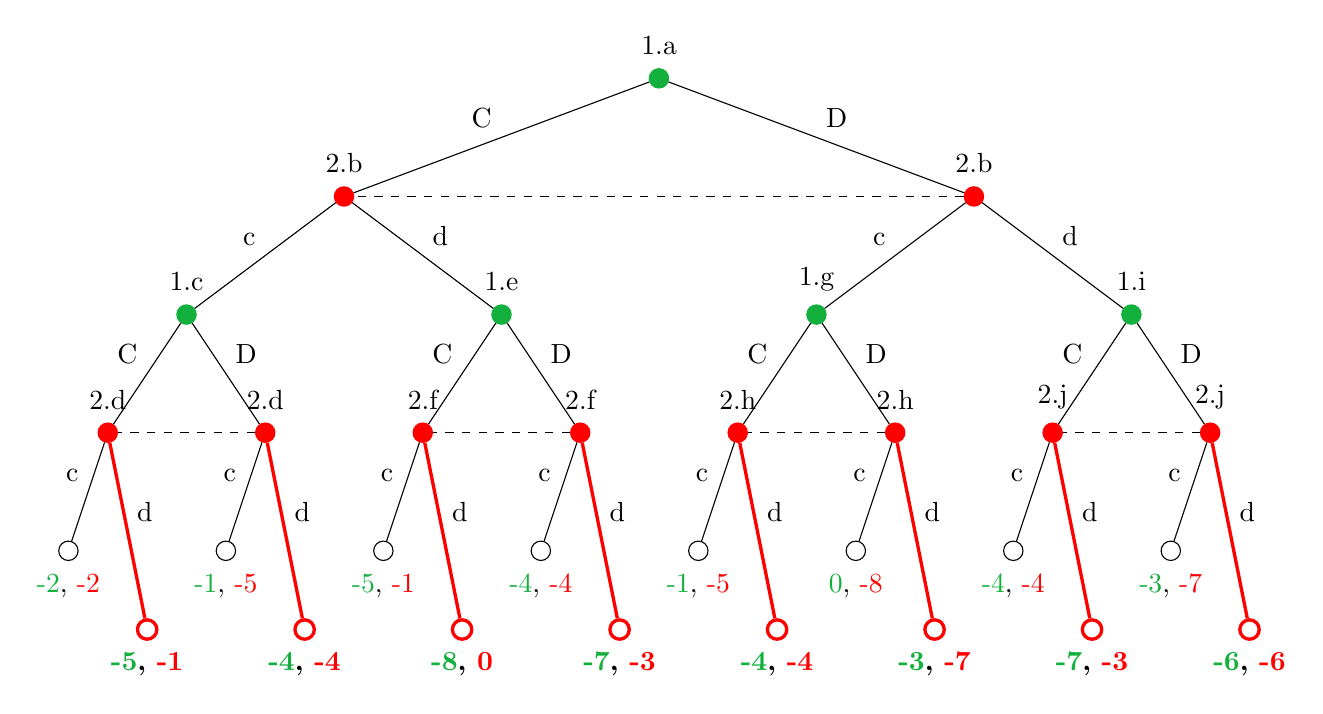
\begin{tikzpicture}
\node[noeud-std, color=green] (n1) {}
   [sibling distance=8cm]
      child {node[noeud-std, color=red] (n2-1c) {} % 1
      [sibling distance=4cm]
             child{node[noeud-std, color=green] (n1-1c2c){} % 2
                [sibling distance=2cm]
                child{node[noeud-std, color=red] (n2-1c2c1c){}  % 1
                    [sibling distance = 1cm]
                         child[level distance=1.5cm]{node[noeud-std,fill=white] (p-1c2c1c2c){} } % 1
                         child[level distance=2.5cm, very thick, red]{node[noeud-std,fill=white] (p-1c2c1c2d){} } % 1
                     }
                child{node[noeud-std, color=red] (n2-1c2c1d){}  % 1
                    [sibling distance = 1cm]
                        child[level distance=1.5cm]{node[noeud-std,fill=white] (p-1c2c1d2c){} } % 1
                        child[level distance=2.5cm, very thick, red]{node[noeud-std,fill=white] (p-1c2c1d2d){} } % 1
                    }
            }
            child{node[noeud-std, color=green] (n1-1c2d){} % 2
                [sibling distance=2cm]
                child{node[noeud-std, color=red] (n2-1c2d1c){}  % 1
                    [sibling distance = 1cm]
                         child[level distance=1.5cm]{node[noeud-std,fill=white] (p-1c2d1c2c){} } % 1
                         child[level distance=2.5cm, very thick, red]{node[noeud-std,fill=white] (p-1c2d1c2d){} } % 1
                     }
                child{node[noeud-std, color=red] (n2-1c2d1d){}  % 1
                    [sibling distance = 1cm]
                        child[level distance=1.5cm]{node[noeud-std,fill=white] (p-1c2d1d2c){} } % 1
                        child[level distance=2.5cm, very thick, red]{node[noeud-std,fill=white] (p-1c2d1d2d){} } % 1
                    }
            }
   }
   child {node[noeud-std, color=red] (n2-1d) {} % 1
      [sibling distance=4cm]
             child{node[noeud-std, color=green] (n1-1d2c){} % 2
                [sibling distance=2cm]
                child{node[noeud-std, color=red] (n2-1d2c1c){}  % 1
                    [sibling distance = 1cm]
                         child[level distance=1.5cm]{node[noeud-std,fill=white] (p-1d2c1c2c){} } % 1
                         child[level distance=2.5cm, very thick, red]{node[noeud-std,fill=white] (p-1d2c1c2d){} } % 1
                     }
                child{node[noeud-std, color=red] (n2-1d2c1d){}  % 1
                    [sibling distance = 1cm]
                        child[level distance=1.5cm]{node[noeud-std,fill=white] (p-1d2c1d2c){} } % 1
                        child[level distance=2.5cm, very thick, red]{node[noeud-std,fill=white] (p-1d2c1d2d){} } % 1
                    }
            }
            child{node[noeud-std, color=green] (n1-1d2d){} % 2
                [sibling distance=2cm]
                child{node[noeud-std, color=red] (n2-1d2d1c){}  % 1
                    [sibling distance = 1cm]
                         child[level distance=1.5cm]{node[noeud-std,fill=white] (p-1d2d1c2c){} } % 1
                         child[level distance=2.5cm, very thick, red]{node[noeud-std,fill=white] (p-1d2d1c2d){} } % 1
                     }
                child{node[noeud-std, color=red] (n2-1d2d1d){}  % 1
                    [sibling distance = 1cm]
                        child[level distance=1.5cm]{node[noeud-std,fill=white] (p-1d2d1d2c){} } % 1
                        child[level distance=2.5cm, very thick, red]{node[noeud-std,fill=white] (p-1d2d1d2d){} } % 1
                    }
            }
   }

;
%
\node[above=5pt] at (n1) {1.a};
\node[above left] at ($(n1)!{0.5}!(n2-1c)$) {C};
\node[above right] at ($(n1)!{0.5}!(n2-1d)$) {D};

\node[above=5pt] at (n2-1c) {2.b};
\node[above left] at ($(n2-1c)!{0.5}!(n1-1c2c)$) {c};
\node[above right] at ($(n2-1c)!{0.5}!(n1-1c2d)$) {d};
\node[above=5pt] at (n1-1c2c) {1.c};
\node[above left] at ($(n1-1c2c)!{0.5}!(n2-1c2c1c)$) {C};
\node[above right] at ($(n1-1c2c)!{0.5}!(n2-1c2c1d)$) {D};
\node[above=5pt] at (n2-1c2c1d) {2.d};
\node[above left] at ($(n2-1c2c1d)!{0.5}!(p-1c2c1d2c)$) {c};
\node[above right] at ($(n2-1c2c1d)!{0.5}!(p-1c2c1d2d)$) {d};
\node[above=5pt] at (n2-1c2c1c) {2.d};
\node[above left] at ($(n2-1c2c1c)!{0.5}!(p-1c2c1c2c)$) {c};
\node[above right] at ($(n2-1c2c1c)!{0.5}!(p-1c2c1c2d)$) {d};
\node[above=5pt] at (n1-1c2d) {1.e};
\node[above left] at ($(n1-1c2d)!{0.5}!(n2-1c2d1c)$) {C};
\node[above right] at ($(n1-1c2d)!{0.5}!(n2-1c2d1d)$) {D};
\node[above=5pt] at (n2-1c2d1d) {2.f};
\node[above left] at ($(n2-1c2d1d)!{0.5}!(p-1c2d1d2c)$) {c};
\node[above right] at ($(n2-1c2d1d)!{0.5}!(p-1c2d1d2d)$) {d};
\node[above=5pt] at (n2-1c2d1c) {2.f};
\node[above left] at ($(n2-1c2d1c)!{0.5}!(p-1c2d1c2c)$) {c};
\node[above right] at ($(n2-1c2d1c)!{0.5}!(p-1c2d1c2d)$) {d};

\node[above=5pt] at (n2-1d) {2.b};
\node[above left] at ($(n2-1d)!{0.5}!(n1-1d2c)$) {c};
\node[above right] at ($(n2-1d)!{0.5}!(n1-1d2d)$) {d};
\node[above=5pt] at (n1-1d2c) {1.g};
\node[above left] at ($(n1-1d2c)!{0.5}!(n2-1d2c1c)$) {C};
\node[above right] at ($(n1-1d2c)!{0.5}!(n2-1d2c1d)$) {D};
\node[above=5pt] at (n2-1d2c1d) {2.h};
\node[above left] at ($(n2-1d2c1d)!{0.5}!(p-1d2c1d2c)$) {c};
\node[above right] at ($(n2-1d2c1d)!{0.5}!(p-1d2c1d2d)$) {d};
\node[above=5pt] at (n2-1d2c1c) {2.h};
\node[above left] at ($(n2-1d2c1c)!{0.5}!(p-1d2c1c2c)$) {c};
\node[above right] at ($(n2-1d2c1c)!{0.5}!(p-1d2c1c2d)$) {d};
\node[above=5pt] at (n1-1d2d) {1.i};
\node[above left] at ($(n1-1d2d)!{0.5}!(n2-1d2d1c)$) {C};
\node[above right] at ($(n1-1d2d)!{0.5}!(n2-1d2d1d)$) {D};
\node[above=5pt] at (n2-1d2d1d) {2.j};
\node[above left] at ($(n2-1d2d1d)!{0.5}!(p-1d2d1d2c)$) {c};
\node[above right] at ($(n2-1d2d1d)!{0.5}!(p-1d2d1d2d)$) {d};
\node[above=5pt] at (n2-1d2d1c) {2.j};
\node[above left] at ($(n2-1d2d1c)!{0.5}!(p-1d2d1c2c)$) {c};
\node[above right] at ($(n2-1d2d1c)!{0.5}!(p-1d2d1c2d)$) {d};

\path (n2-1d)  edge [dashed] node {} (n2-1c);
\path (n2-1c2c1d)  edge [dashed] node {} (n2-1c2c1c);
\path (n2-1c2d1d)  edge [dashed] node {} (n2-1c2d1c);
\path (n2-1d2c1d)  edge [dashed] node {} (n2-1d2c1c);
\path (n2-1d2d1d)  edge [dashed] node {} (n2-1d2d1c);

\node[below = 5pt] at ($(p-1c2c1c2c)$) {\payoff{-2}{-2}};
\node[below = 5pt] at ($(p-1c2c1c2d)$) {\textbf{\payoff{-5}{-1}}};
\node[below = 5pt] at ($(p-1c2c1d2c)$) {\payoff{-1}{-5}};
\node[below = 5pt] at ($(p-1c2c1d2d)$) {\textbf{\payoff{-4}{-4}}};


\node[below = 5pt] at ($(p-1c2d1c2c)$) {\payoff{-5}{-1}};
\node[below = 5pt] at ($(p-1c2d1c2d)$) {\textbf{\payoff{-8}{0}}};
\node[below = 5pt] at ($(p-1c2d1d2c)$) {\payoff{-4}{-4}};
\node[below = 5pt] at ($(p-1c2d1d2d)$) {\textbf{\payoff{-7}{-3}}};


\node[below = 5pt] at ($(p-1d2c1c2c)$) {\payoff{-1}{-5}};
\node[below = 5pt] at ($(p-1d2c1c2d)$) {\textbf{\payoff{-4}{-4}}};
\node[below = 5pt] at ($(p-1d2c1d2c)$) {\payoff{0}{-8}};
\node[below = 5pt] at ($(p-1d2c1d2d)$) {\textbf{\payoff{-3}{-7}}};


\node[below = 5pt] at ($(p-1d2d1c2c)$) {\payoff{-4}{-4}};
\node[below = 5pt] at ($(p-1d2d1c2d)$) {\textbf{\payoff{-7}{-3}}};
\node[below = 5pt] at ($(p-1d2d1d2c)$) {\payoff{-3}{-7}};
\node[below = 5pt] at ($(p-1d2d1d2d)$) {\textbf{\payoff{-6}{-6}}};

\end{tikzpicture}}
\caption{Repeated Prisoner's Dilemma: backward induction step 1.}
\end{figure}

\end{frame}

\begin{frame}{Nash equilibrium: backward induction (2)}
    \begin{figure}[!ht]
    \centering
    \scalebox{0.65}{
    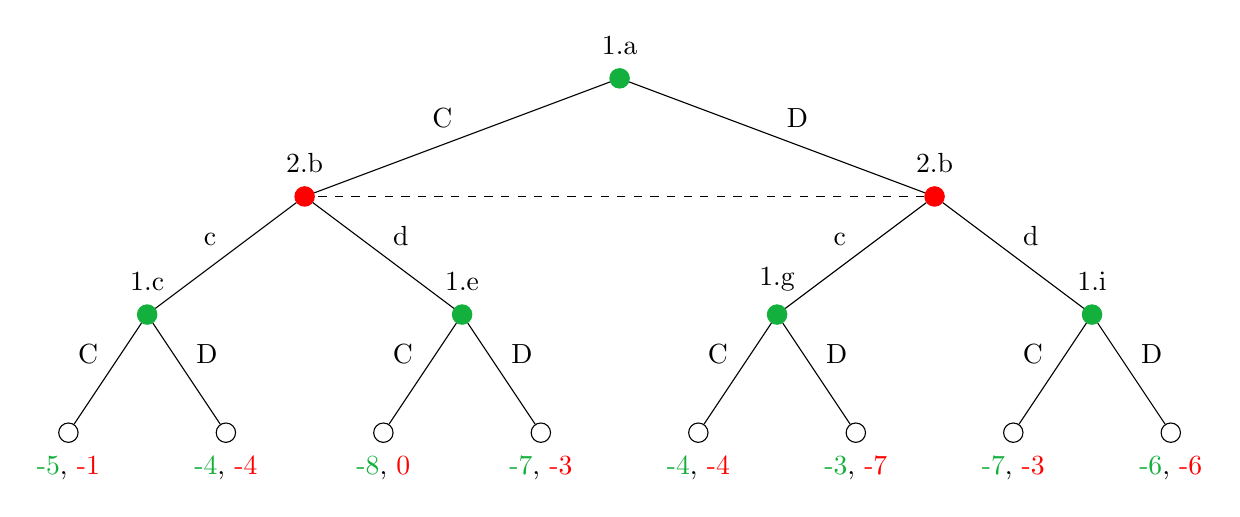
\begin{tikzpicture}
        \node[noeud-std, color=green] (n1) {}
           [sibling distance=8cm]
              child {node[noeud-std, color=red] (n2-1c) {} % 1
              [sibling distance=4cm]
                     child{node[noeud-std, color=green] (n1-1c2c){} % 2
                        [sibling distance=2cm]
                        child{node[noeud-std, fill=white] (n2-1c2c1c){}}
                        child{node[noeud-std, fill=white] (n2-1c2c1d){}}
                    }
                    child{node[noeud-std, color=green] (n1-1c2d){} % 2
                        [sibling distance=2cm]
                        child{node[noeud-std, fill=white] (n2-1c2d1c){}}
                        child{node[noeud-std, fill=white] (n2-1c2d1d){}}
                    }
           }
           child {node[noeud-std, color=red] (n2-1d) {} % 1
              [sibling distance=4cm]
                     child{node[noeud-std, color=green] (n1-1d2c){} % 2
                        [sibling distance=2cm]
                        child{node[noeud-std, fill=white] (n2-1d2c1c){}}
                        child{node[noeud-std, fill=white] (n2-1d2c1d){}}
                    }
                    child{node[noeud-std, color=green] (n1-1d2d){} % 2
                        [sibling distance=2cm]
                        child{node[noeud-std, fill=white] (n2-1d2d1c){}}
                        child{node[noeud-std, fill=white] (n2-1d2d1d){}}
                    }
           }
        ;
        %
        \node[above=5pt] at (n1) {1.a};
        \node[above left] at ($(n1)!{0.5}!(n2-1c)$) {C};
        \node[above right] at ($(n1)!{0.5}!(n2-1d)$) {D};

        \node[above=5pt] at (n2-1c) {2.b};
        \node[above left] at ($(n2-1c)!{0.5}!(n1-1c2c)$) {c};
        \node[above right] at ($(n2-1c)!{0.5}!(n1-1c2d)$) {d};
        \node[above=5pt] at (n1-1c2c) {1.c};
        \node[above left] at ($(n1-1c2c)!{0.5}!(n2-1c2c1c)$) {C};
        \node[above right] at ($(n1-1c2c)!{0.5}!(n2-1c2c1d)$) {D};
        \node[above=5pt] at (n1-1c2d) {1.e};
        \node[above left] at ($(n1-1c2d)!{0.5}!(n2-1c2d1c)$) {C};
        \node[above right] at ($(n1-1c2d)!{0.5}!(n2-1c2d1d)$) {D};

        \node[above=5pt] at (n2-1d) {2.b};
        \node[above left] at ($(n2-1d)!{0.5}!(n1-1d2c)$) {c};
        \node[above right] at ($(n2-1d)!{0.5}!(n1-1d2d)$) {d};
        \node[above=5pt] at (n1-1d2c) {1.g};
        \node[above left] at ($(n1-1d2c)!{0.5}!(n2-1d2c1c)$) {C};
        \node[above right] at ($(n1-1d2c)!{0.5}!(n2-1d2c1d)$) {D};
        \node[above=5pt] at (n1-1d2d) {1.i};
        \node[above left] at ($(n1-1d2d)!{0.5}!(n2-1d2d1c)$) {C};
        \node[above right] at ($(n1-1d2d)!{0.5}!(n2-1d2d1d)$) {D};

        \path (n2-1d)  edge [dashed] node {} (n2-1c);

        \node[below = 5pt] at ($(n2-1c2c1c)$) {\payoff{-5}{-1}};
        \node[below = 5pt] at ($(n2-1c2c1d)$) {\payoff{-4}{-4}};

        \node[below = 5pt] at ($(n2-1c2d1c)$) {\payoff{-8}{0}};
        \node[below = 5pt] at ($(n2-1c2d1d)$) {\payoff{-7}{-3}};

        \node[below = 5pt] at ($(n2-1d2c1c)$) {\payoff{-4}{-4}};
        \node[below = 5pt] at ($(n2-1d2c1d)$) {\payoff{-3}{-7}};

        \node[below = 5pt] at ($(n2-1d2d1c)$) {\payoff{-7}{-3}};
        \node[below = 5pt] at ($(n2-1d2d1d)$) {\payoff{-6}{-6}};
    \end{tikzpicture}}
    \caption{Repeated Prisoner's Dilemma: backward induction step 2.}
    \end{figure}
\end{frame}

\begin{frame}{Nash equilibrium: backward induction (3)}
    \begin{figure}[!ht]
    \centering
    \scalebox{0.65}{
    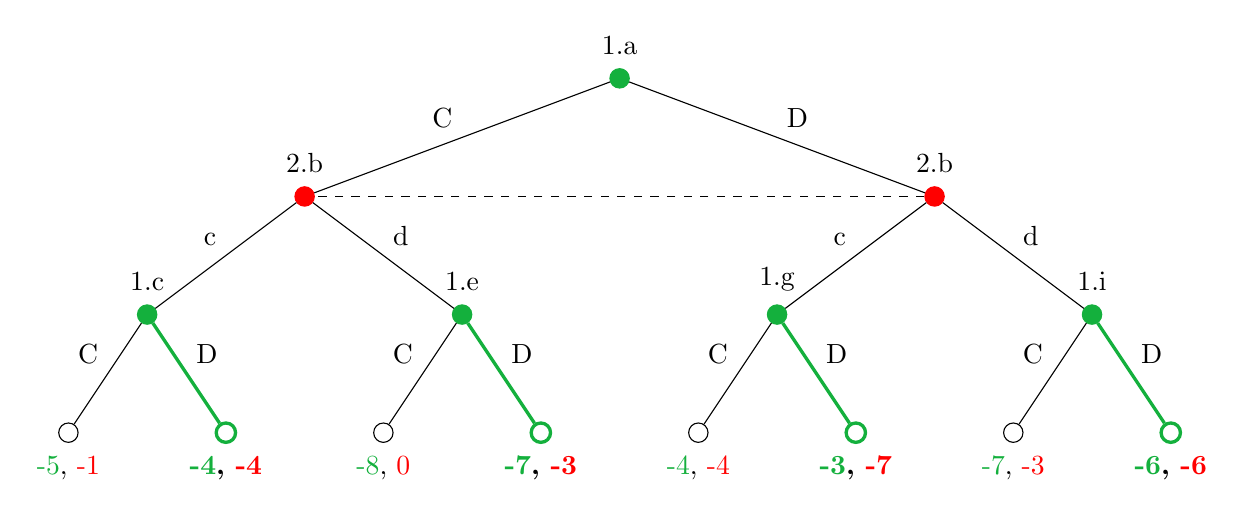
\begin{tikzpicture}
        \node[noeud-std, color=green] (n1) {}
           [sibling distance=8cm]
              child {node[noeud-std, color=red] (n2-1c) {} % 1
              [sibling distance=4cm]
                     child{node[noeud-std, color=green] (n1-1c2c){} % 2
                        [sibling distance=2cm]
                        child{node[noeud-std, fill=white] (n2-1c2c1c){}}
                        child[very thick, green]{node[noeud-std, fill=white] (n2-1c2c1d){}}
                    }
                    child{node[noeud-std, color=green] (n1-1c2d){} % 2
                        [sibling distance=2cm]
                        child{node[noeud-std, fill=white] (n2-1c2d1c){}}
                        child[very thick, green]{node[noeud-std, fill=white] (n2-1c2d1d){}}
                    }
           }
           child {node[noeud-std, color=red] (n2-1d) {} % 1
              [sibling distance=4cm]
                     child{node[noeud-std, color=green] (n1-1d2c){} % 2
                        [sibling distance=2cm]
                        child{node[noeud-std, fill=white] (n2-1d2c1c){}}
                        child[very thick, green]{node[noeud-std, fill=white] (n2-1d2c1d){}}
                    }
                    child{node[noeud-std, color=green] (n1-1d2d){} % 2
                        [sibling distance=2cm]
                        child{node[noeud-std, fill=white] (n2-1d2d1c){}}
                        child[very thick, green]{node[noeud-std, fill=white] (n2-1d2d1d){}}
                    }
           }
        ;
        %
        \node[above=5pt] at (n1) {1.a};
        \node[above left] at ($(n1)!{0.5}!(n2-1c)$) {C};
        \node[above right] at ($(n1)!{0.5}!(n2-1d)$) {D};

        \node[above=5pt] at (n2-1c) {2.b};
        \node[above left] at ($(n2-1c)!{0.5}!(n1-1c2c)$) {c};
        \node[above right] at ($(n2-1c)!{0.5}!(n1-1c2d)$) {d};
        \node[above=5pt] at (n1-1c2c) {1.c};
        \node[above left] at ($(n1-1c2c)!{0.5}!(n2-1c2c1c)$) {C};
        \node[above right] at ($(n1-1c2c)!{0.5}!(n2-1c2c1d)$) {D};
        \node[above=5pt] at (n1-1c2d) {1.e};
        \node[above left] at ($(n1-1c2d)!{0.5}!(n2-1c2d1c)$) {C};
        \node[above right] at ($(n1-1c2d)!{0.5}!(n2-1c2d1d)$) {D};

        \node[above=5pt] at (n2-1d) {2.b};
        \node[above left] at ($(n2-1d)!{0.5}!(n1-1d2c)$) {c};
        \node[above right] at ($(n2-1d)!{0.5}!(n1-1d2d)$) {d};
        \node[above=5pt] at (n1-1d2c) {1.g};
        \node[above left] at ($(n1-1d2c)!{0.5}!(n2-1d2c1c)$) {C};
        \node[above right] at ($(n1-1d2c)!{0.5}!(n2-1d2c1d)$) {D};
        \node[above=5pt] at (n1-1d2d) {1.i};
        \node[above left] at ($(n1-1d2d)!{0.5}!(n2-1d2d1c)$) {C};
        \node[above right] at ($(n1-1d2d)!{0.5}!(n2-1d2d1d)$) {D};

        \path (n2-1d)  edge [dashed] node {} (n2-1c);

        \node[below = 5pt] at ($(n2-1c2c1c)$) {\payoff{-5}{-1}};
        \node[below = 5pt] at ($(n2-1c2c1d)$) {\textbf{\payoff{-4}{-4}}};

        \node[below = 5pt] at ($(n2-1c2d1c)$) {\payoff{-8}{0}};
        \node[below = 5pt] at ($(n2-1c2d1d)$) {\textbf{\payoff{-7}{-3}}};

        \node[below = 5pt] at ($(n2-1d2c1c)$) {\payoff{-4}{-4}};
        \node[below = 5pt] at ($(n2-1d2c1d)$) {\textbf{\payoff{-3}{-7}}};

        \node[below = 5pt] at ($(n2-1d2d1c)$) {\payoff{-7}{-3}};
        \node[below = 5pt] at ($(n2-1d2d1d)$) {\textbf{\payoff{-6}{-6}}};
    \end{tikzpicture}}
    \caption{Repeated Prisoner's Dilemma: backward induction step 3.}
    \end{figure}
\end{frame}

\begin{frame}{Nash equilibrium: backward induction (4)}
    \begin{figure}[!ht]
        \centering
        \scalebox{0.65}{
        \begin{tikzpicture}
            \node[noeud-std, color=green] (n1) {}
               [sibling distance=8cm]
                  child {node[noeud-std, color=red] (n2-1c) {} % 1
                  [sibling distance=4cm]
                        child{node[noeud-std, fill=white] (n1-1c2c){}}
                        child{node[noeud-std, fill=white] (n1-1c2d){}}
               }
               child {node[noeud-std, color=red] (n2-1d) {} % 1
                  [sibling distance=4cm]
                        child{node[noeud-std, fill=white] (n1-1d2c){}}
                        child{node[noeud-std, fill=white] (n1-1d2d){}}
               }
            ;
            %
            \node[above=5pt] at (n1) {1.a};
            \node[above left] at ($(n1)!{0.5}!(n2-1c)$) {C};
            \node[above right] at ($(n1)!{0.5}!(n2-1d)$) {D};

            \node[above=5pt] at (n2-1c) {2.b};
            \node[above left] at ($(n2-1c)!{0.5}!(n1-1c2c)$) {c};
            \node[above right] at ($(n2-1c)!{0.5}!(n1-1c2d)$) {d};

            \node[above=5pt] at (n2-1d) {2.b};
            \node[above left] at ($(n2-1d)!{0.5}!(n1-1d2c)$) {c};
            \node[above right] at ($(n2-1d)!{0.5}!(n1-1d2d)$) {d};

            \path (n2-1d)  edge [dashed] node {} (n2-1c);

            \node[below = 5pt] at ($(n1-1c2c)$) {\payoff{-4}{-4}};
            \node[below = 5pt] at ($(n1-1c2d)$) {\payoff{-7}{-3}};
            \node[below = 5pt] at ($(n1-1d2c)$) {\payoff{-3}{-7}};
            \node[below = 5pt] at ($(n1-1d2d)$) {\payoff{-6}{-6}};
        \end{tikzpicture}}
        \caption{Repeated Prisoner's Dilemma: backward induction step 4.}
    \end{figure}
\end{frame}

\begin{frame}{Nash equilibrium: backward induction (5)}
    \begin{figure}[!ht]
        \centering
        \scalebox{0.65}{
        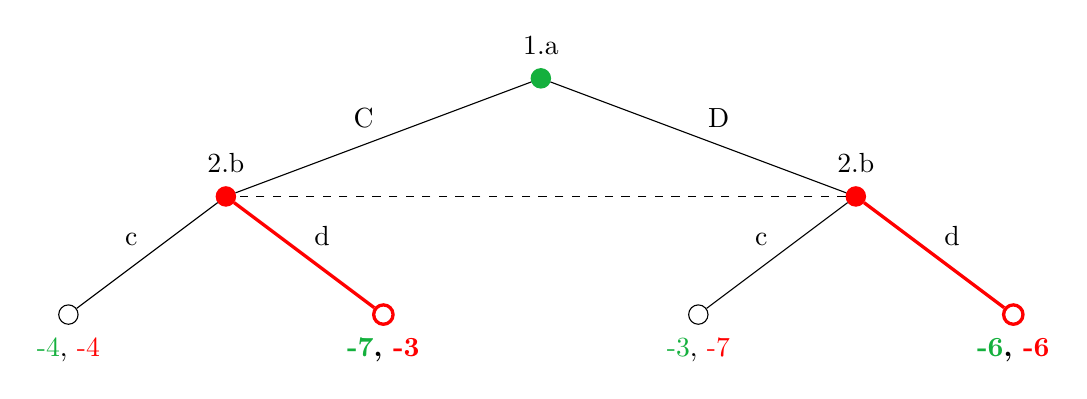
\begin{tikzpicture}
            \node[noeud-std, color=green] (n1) {}
               [sibling distance=8cm]
                  child {node[noeud-std, color=red] (n2-1c) {} % 1
                  [sibling distance=4cm]
                        child{node[noeud-std, fill=white] (n1-1c2c){}}
                        child[very thick, red]{node[noeud-std, fill=white] (n1-1c2d){}}
               }
               child {node[noeud-std, color=red] (n2-1d) {} % 1
                  [sibling distance=4cm]
                        child{node[noeud-std, fill=white] (n1-1d2c){}}
                        child[very thick, red]{node[noeud-std, fill=white] (n1-1d2d){}}
               }
            ;
            %
            \node[above=5pt] at (n1) {1.a};
            \node[above left] at ($(n1)!{0.5}!(n2-1c)$) {C};
            \node[above right] at ($(n1)!{0.5}!(n2-1d)$) {D};

            \node[above=5pt] at (n2-1c) {2.b};
            \node[above left] at ($(n2-1c)!{0.5}!(n1-1c2c)$) {c};
            \node[above right] at ($(n2-1c)!{0.5}!(n1-1c2d)$) {d};

            \node[above=5pt] at (n2-1d) {2.b};
            \node[above left] at ($(n2-1d)!{0.5}!(n1-1d2c)$) {c};
            \node[above right] at ($(n2-1d)!{0.5}!(n1-1d2d)$) {d};

            \path (n2-1d)  edge [dashed] node {} (n2-1c);

            \node[below = 5pt] at ($(n1-1c2c)$) {\payoff{-4}{-4}};
            \node[below = 5pt] at ($(n1-1c2d)$) {\textbf{\payoff{-7}{-3}}};
            \node[below = 5pt] at ($(n1-1d2c)$) {\payoff{-3}{-7}};
            \node[below = 5pt] at ($(n1-1d2d)$) {\textbf{\payoff{-6}{-6}}};
        \end{tikzpicture}}
        \caption{Repeated Prisoner's Dilemma: backward induction step 5.}
    \end{figure}
\end{frame}

\begin{frame}{Nash equilibrium: backward induction (6)}
    \begin{figure}[!ht]
        \centering
        \scalebox{0.65}{
        \begin{tikzpicture}
            \node[noeud-std, color=green] (n1) {}
                [sibling distance=8cm]
                    child {node[noeud-std, fill=white] (n2-1c) {}}
                    child {node[noeud-std, fill=white] (n2-1d) {} }
            ;
            %
            \node[above=5pt] at (n1) {1.a};
            \node[above left] at ($(n1)!{0.5}!(n2-1c)$) {C};
            \node[above right] at ($(n1)!{0.5}!(n2-1d)$) {D};

            \node[below = 5pt] at ($(n2-1c)$) {\payoff{-7}{-3}};
            \node[below = 5pt] at ($(n2-1d)$) {\payoff{-6}{-6}};
        \end{tikzpicture}}
        \caption{Repeated Prisoner's Dilemma: backward induction step 6.}
    \end{figure}
\end{frame}

\begin{frame}{Nash equilibrium: backward induction (7)}
    \begin{figure}[!ht]
        \centering
        \scalebox{0.65}{
        \begin{tikzpicture}
            \node[noeud-std, color=green] (n1) {}
                [sibling distance=8cm]
                    child {node[noeud-std, fill=white] (n2-1c) {}}
                    child[very thick, green] {node[noeud-std, fill=white] (n2-1d) {} }
            ;
            %
            \node[above=5pt] at (n1) {1.a};
            \node[above left] at ($(n1)!{0.5}!(n2-1c)$) {C};
            \node[above right] at ($(n1)!{0.5}!(n2-1d)$) {D};

            \node[below = 5pt] at ($(n2-1c)$) {\payoff{-7}{-3}};
            \node[below = 5pt] at ($(n2-1d)$) {\textbf{\payoff{-6}{-6}}};
        \end{tikzpicture}}
        \caption{Repeated Prisoner's Dilemma: backward induction step 7.}
    \end{figure}

    \begin{block}{Conclusion}
        The only Nash Equilibrium is for both players to defect at each round, leading
        to the total payoff (\payoff{-6}{-6}).
    \end{block}
\end{frame}

\begin{frame}{Take-home message \#1 and social experiments}
    \metroset{block=fill}
    \begin{block}{Take-home message \#1}
        Repeating the same game $K$ times where $K$ is known by the players before the game starts
        \textbf{do not} change the Nash equilibrium.\\\
        
        Proof? Use backward induction.
    \end{block}

    %\vspace{1cm}
    %\textbf{{\color{orange}Does this prediction match actual human behaviour?}}\\
    %No, experiments show that cooperation often appears in finitely repeated Prisoner's
    %Dilemma, contradicting backward induction\footnote{See for example
    %Matthew Embrey, Guillaume R. Fréchette, and Segvi Yuksel, \textbf{Cooperation in the
    %finitely repeated Prisoner's Dilemma}, {\color{gray}\textit{The Quarterly Journal of Economics},
    %509--511, 2018}.}.
\end{frame}

\note{
    Could be interesting to ask the audience to remember the take-home messages because
    we will randomly pick people among them at the end to check their memory.

    About the match with actual human behaviors, might be cool to reassure the audience
    on the results of their game if cooperation indeed appeared in the example.

    As an anecdote, the cited paper has "We are responsible for all errors" written in a
    footnote on the first page. I personally never saw that before.
}


\section{Infinitely Repeated Games}
\begin{frame}{Outline}
    \tableofcontents[currentsection]
\end{frame}

\begin{frame}{Let's again play the repeated Prisoner's Dilemma}
    \begin{exampleblock}{Example}
        Consider again the Prisoner's Dilemma in normal form.
        \begin{table}
            \begin{tabular}{c|cc}
                & {\color{red}c}    & {\color{red}d} \\
                \hline
                {\color{green}C}    & \payoff{-1}{-1}   & \payoff{-4}{~0} \\
                {\color{green}D}    & \payoff{~0}{-4}    & \payoff{-3}{-3} 
            \end{tabular}
            \caption{Prisoner's Dilemma in normal form.}
        \end{table}
    
        We will roll a (fair) dice after each round
        \begin{itemize}
            \item if the result is 1, the game stops,
            \item otherwise the game continues.
        \end{itemize}
        At the end of each round, you collect your payoff (and thus observe what
        the other has played).
    \end{exampleblock}
\end{frame}

\note{
    Stress that this game will be used during the whole presentation so that they should
    try to remember it.

    Ask the audience if they would change their strategy w.r.t. the previous game.
}

\begin{frame}{Can a cooperative strategy be a Nash Equilibrium?}
    \begin{block}{Cooperative strategy}
        \textit{Cooperate at each round, until the other defect,
        then defect forever} and assume both players play accordingly.
    \end{block}

    \begin{exampleblock}{For this to be a Nash Equilibrium...}
        Neither player can expect to gain by any unilateral deviation at any point
        in time (i.e., for any history of past moves).
        
        Two possible history of past moves in this case
        \begin{enumerate}
            \pause
            \item \textbf{one of the player has defected in the past}: both players are then always defecting
            and neither player could gain by deviating alone to cooperation, \pause
            \item \textbf{neither player has ever defected in the past}: both players are then always
            cooperating.
            Could it be more profitable for one player to defect? Less obvious, see blackboard!
        \end{enumerate}
    \end{exampleblock}
\end{frame}
    
\note{
    The total number of rounds follows a geometric distribution with expected value 6. That is, the
    probability that we play \textit{exactly} $k$ rounds is given by
    \[ p(k) = \left(\frac{5}{6}\right)^{k-1}\frac{1}{6}. \]

    The following formula is useful in the following reasoning
    \[ \sum_{k=1}^{\infty} kz^k = \frac{z}{(1-z)^2}. \]
}

\note{
    If both players follows the strategy and cooperate, they will each get an expected total future
    payoff of
    \begin{align*}
        \sum_{k=1}^{\infty} (-1k)\cdot p(k) &= -\frac{1}{6} \sum_{k=1}^{\infty} k\left(\frac{5}{6}\right)^{k-1}\\
                                            &= -\frac{1}{5} \sum_{k=1}^{\infty} k\left(\frac{5}{6}\right)^k \\
                                            &= -\frac{1}{5} \frac{5/6}{(1-5/6)^2} \\
                                            &= -\frac{1}{5} \frac{5}{6}\cdot 36 \\
                                            &= -6.
    \end{align*}
}

\note{
    If one of the players deviate and decide to defect, he will get 0 first and then -3 forever because the
    other player will always defect to punish him, the deviating player will then get an expected total future
    payoff of
    \begin{align*}
        0 + \sum_{k=1}^{\infty} (-3)(k-1)\cdot p(k)
        &= -\frac{1}{2} \sum_{k=2}^{\infty} (k-1)\left(\frac{5}{6}\right)^{k-1} \\
        &= -\frac{1}{2} \sum_{k'=1}^{\infty} k'\left(\frac{5}{6}\right)^{k'} \\
        &= -15 < -6.
    \end{align*}
}

\begin{frame}{Interpretation of the cooperative Nash Equilibrium}
    \begin{exampleblock}{How can we explain this cooperative equilibrium?}
        \begin{itemize}
            \item At each round, both players believe that there is a high probability that they
            will play again. The hope of \textbf{inducing a future cooperative behavior by the other
            player} can give each player an incentive to be generous.
            \item In addition, both players know that \textbf{defecting is} forever \textbf{punished} by
            the other player so that defecting, while more profitable in the short-term, is not profitable
            in the long-term.
        \end{itemize}
    \end{exampleblock}
\end{frame}

\begin{frame}{Take-home message \#2}
    \metroset{block=fill}
    \begin{block}{Take-home-message \#2}
        Rational behavior in a repeated game with a potentially infinite time horizon may be
        very different from rational behavior in the corresponding game played once (or a finite
        and known number of times).
    \end{block}
\end{frame}


\section{Folk Theorem}
\begin{frame}{Outline}
    \tableofcontents[currentsection]
\end{frame}



\begin{frame}{Folk Theorem}
    \textbf{Folk Theorems}
    \begin{itemize}
        \item Theorems that circulate among mathematicians but cannot be traced back to one individual
        \item Considered to have established status but generally no proof in complete form
        \item One notable one in Game Theory, that we are going to see today
    \end{itemize}
\end{frame}


\begin{frame}{Folk Theorem}
    \textbf{Formulation of the theorem:}\\
    \textit{Consider any $n$-player normal-form game $G$ and any payoff profile $r = (r_1,r_2,...,r_n)$. Then:}
    \begin{enumerate}
        \item \textit{If $r$ is the payoff profile for any Nash equilibrium s of the infinitely repeated $G$ with average rewards, then for each player $i$, $r_i$ is enforceable.}
        \item \textit{If $r$ is both feasible and enforceable, then $r$ is the payoff profile for some Nash equilibrium of the infinitely repeated $G$ with average rewards.}
    \end{enumerate}
    \textit{This version of the theorem is proven in the book [MAS]}
\end{frame}


\begin{frame}{Folk Theorem}
    \textbf{What does it mean?}\\
    \begin{itemize}
        \item The first part of the theorem means that we can enforce any Nash equilibrium of the infinitely-repeated game
        \item The second part states that any payoff profile that is feasible and enforceable is the payoff profile of a Nash equilibrium 
    \end{itemize}
\end{frame}

\begin{frame}{Folk Theorem}
    \textbf{Consequences}\\
    \begin{itemize}
        \item Interesting consequences: apparition of new Nash equilibrium's for certain games
        \item Example: prisoner's dilemna
        \begin{itemize}
            \item If game goes on long enough ($\delta \rightarrow 1$), cooperation of both players becomes a Nash equilibrium
        \end{itemize}
    \end{itemize}
\end{frame}


\section{Learning Rules}
\begin{frame}{Outline}
    \tableofcontents[currentsection]
\end{frame}


\begin{frame}{Learning rules}
    \textbf{Definition}
    \begin{itemize}
        \item Learning strategy: Use of previous information to improve its behavior
        \item Deeply linked with artificial intelligence
    \end{itemize}
\end{frame}

\begin{frame}{Learning rules}
    \textbf{Two types of theories}
    \begin{itemize}
        \item Descriptive theories: theories that attempt to study the way learning takes place in real life
        \item Prescriptive theories: theories that study the way agents \textit{should} react in real life
    \end{itemize}
\end{frame}

\begin{frame}{Descriptive theories}
    \textbf{Properties}
    \begin{itemize}
        \item \textbf{Realism}: There should be a good match between the formal theory and the natural phenomenon being studied
        \item \textbf{Convergence}: The theory should exhibit convergence of the strategy profile to some equilibrium
    \end{itemize}
\end{frame}

\begin{frame}{Prescriptive theories}
    \textbf{Properties}
    \begin{itemize}
        \item \textbf{Safety}: Guarantees the agent at least learning rule its maxmin payoff, or “security value.”
        \item \textbf{Rationality}: Whenever the opponent's learning rule settles on a stationary strategy the agent settles on a best response to that strategy
        \item \textbf{No-regret}: Yields a better result that any pure strategy the agent could have played
    \end{itemize}
\end{frame}

\begin{frame}{Fictitious play}
    \textbf{Fictitious play}
    \begin{itemize}
        \item One of the earliest learning rules 
        \item Instance of model-based learning where learner maintains belief about opponent
        \item Agent believes that his opponent is playing the mixed strategy given by the empirical distribution of the opponent’s previous actions
    \end{itemize}
\end{frame}

\begin{frame}{Fictitious play}
    \begin{algorithm}[H]
         Initialize beliefs about the opponent strategy\;
         \While{true}{
            Play a best response to the assessed strategy of the opponent\\
            Observe the opponent’s actual play and update beliefs accordingly\\
         }
    \caption{Fictitious play algorithm}
    \end{algorithm}
\end{frame}


\begin{frame}{No-regret playing}
    \textbf{Regret}\\
    \textit{Let $\alpha^t$ be the average per-period reward the agent received up to time $t$ and $\alpha^t(s)$ the average per-period reward the agent would have received by playing strategy $s$.}\\
    \textit{The regret an agent experiences at time $t$ for not having played $s$ is $R^t(s)=\alpha^t-\alpha^t(s)$}
\end{frame}

\begin{frame}{No-regret playing}
    \textbf{No-regret learning rule}\\
    \textit{A learning rule exhibits \textbf{no regret} if it guarantees with high probability that the agent will not experience any positive regret}
\end{frame}

\begin{frame}{No-regret playing}
    \textbf{Example of a no-regret strategy: Regret matching}\\
    \begin{itemize}
        \item At each time step each action is chosen with probability consistent to its regret
        \item The strategy of playing strategy $s$ at timestep $t+1$ is equal to:
        \[
            \sigma_i^{t+1}(s)= \frac{R^t(s)}{\sum_{s'\in S_i} R^t(s')}
        \]
    \end{itemize}
\end{frame}



\begin{frame}{References}
    \nocite{*}
    \bibliographystyle{plain}
    \bibliography{biblio}
\end{frame}

\begin{frame}[standout]
    Questions?
\end{frame}

\end{document}
